\documentclass[tikz,border=2pt]{standalone}
\usepackage{amsmath,amssymb}
\usepackage{tikz}

\begin{document}
% Set covering: choose station towns so that every town is within 18 minutes of a station.
% Schematic layout: stations at towns 4 and 5 cover all six towns (dashed = within 18 min).
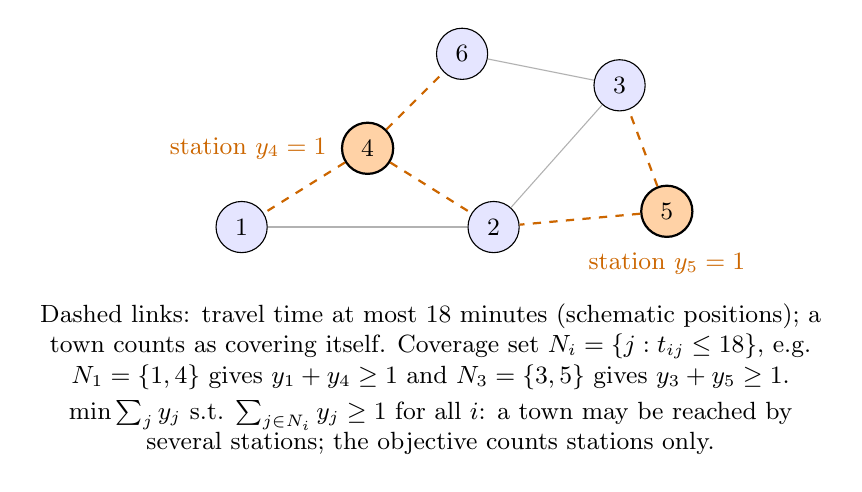
\begin{tikzpicture}[every node/.style={font=\small}, t/.style={draw, circle, fill=blue!10, minimum size=6.5mm, inner sep=0pt}, s/.style={draw, circle, fill=orange!35, minimum size=6.5mm, inner sep=0pt, thick}]
	\node[t] (1) at (0,0) {$1$};
	\node[s] (4) at (1.6,1.0) {$4$};
	\node[t] (2) at (3.2,0.0) {$2$};
	\node[t] (6) at (2.8,2.2) {$6$};
	\node[t] (3) at (4.8,1.8) {$3$};
	\node[s] (5) at (5.4,0.2) {$5$};
	\foreach \a/\b in {4/1, 4/2, 4/6, 5/3, 5/2} {\draw[orange!80!black, dashed, thick] (\a) -- (\b);}
	\draw[gray!60] (1) -- (2); \draw[gray!60] (6) -- (3); \draw[gray!60] (2) -- (3);
	\node[orange!80!black, anchor=east] at (1.2,1.0) {station $y_4=1$};
	\node[orange!80!black, anchor=north] at (5.4,-0.2) {station $y_5=1$};
	\node[anchor=north, align=flush center, text width=10cm] at (2.4,-0.85) {Dashed links: travel time at most $18$ minutes (schematic positions); a town counts as covering itself. Coverage set $N_i=\{j: t_{ij}\le18\}$, e.g. $N_1=\{1,4\}$ gives $y_1+y_4\ge1$ and $N_3=\{3,5\}$ gives $y_3+y_5\ge1$.\\[2pt] $\min\sum_jy_j$ s.t. $\sum_{j\in N_i}y_j\ge1$ for all $i$: a town may be reached by several stations; the objective counts stations only.};
\end{tikzpicture}
\end{document}
